Consider a more practical approach that takes all the previously discussed aspects.
Applying modern frameworks like ASP .NET Core, Angular etc.
let be the following authentication flow as per diagram below
\begin{figure}[H]
    \centering
    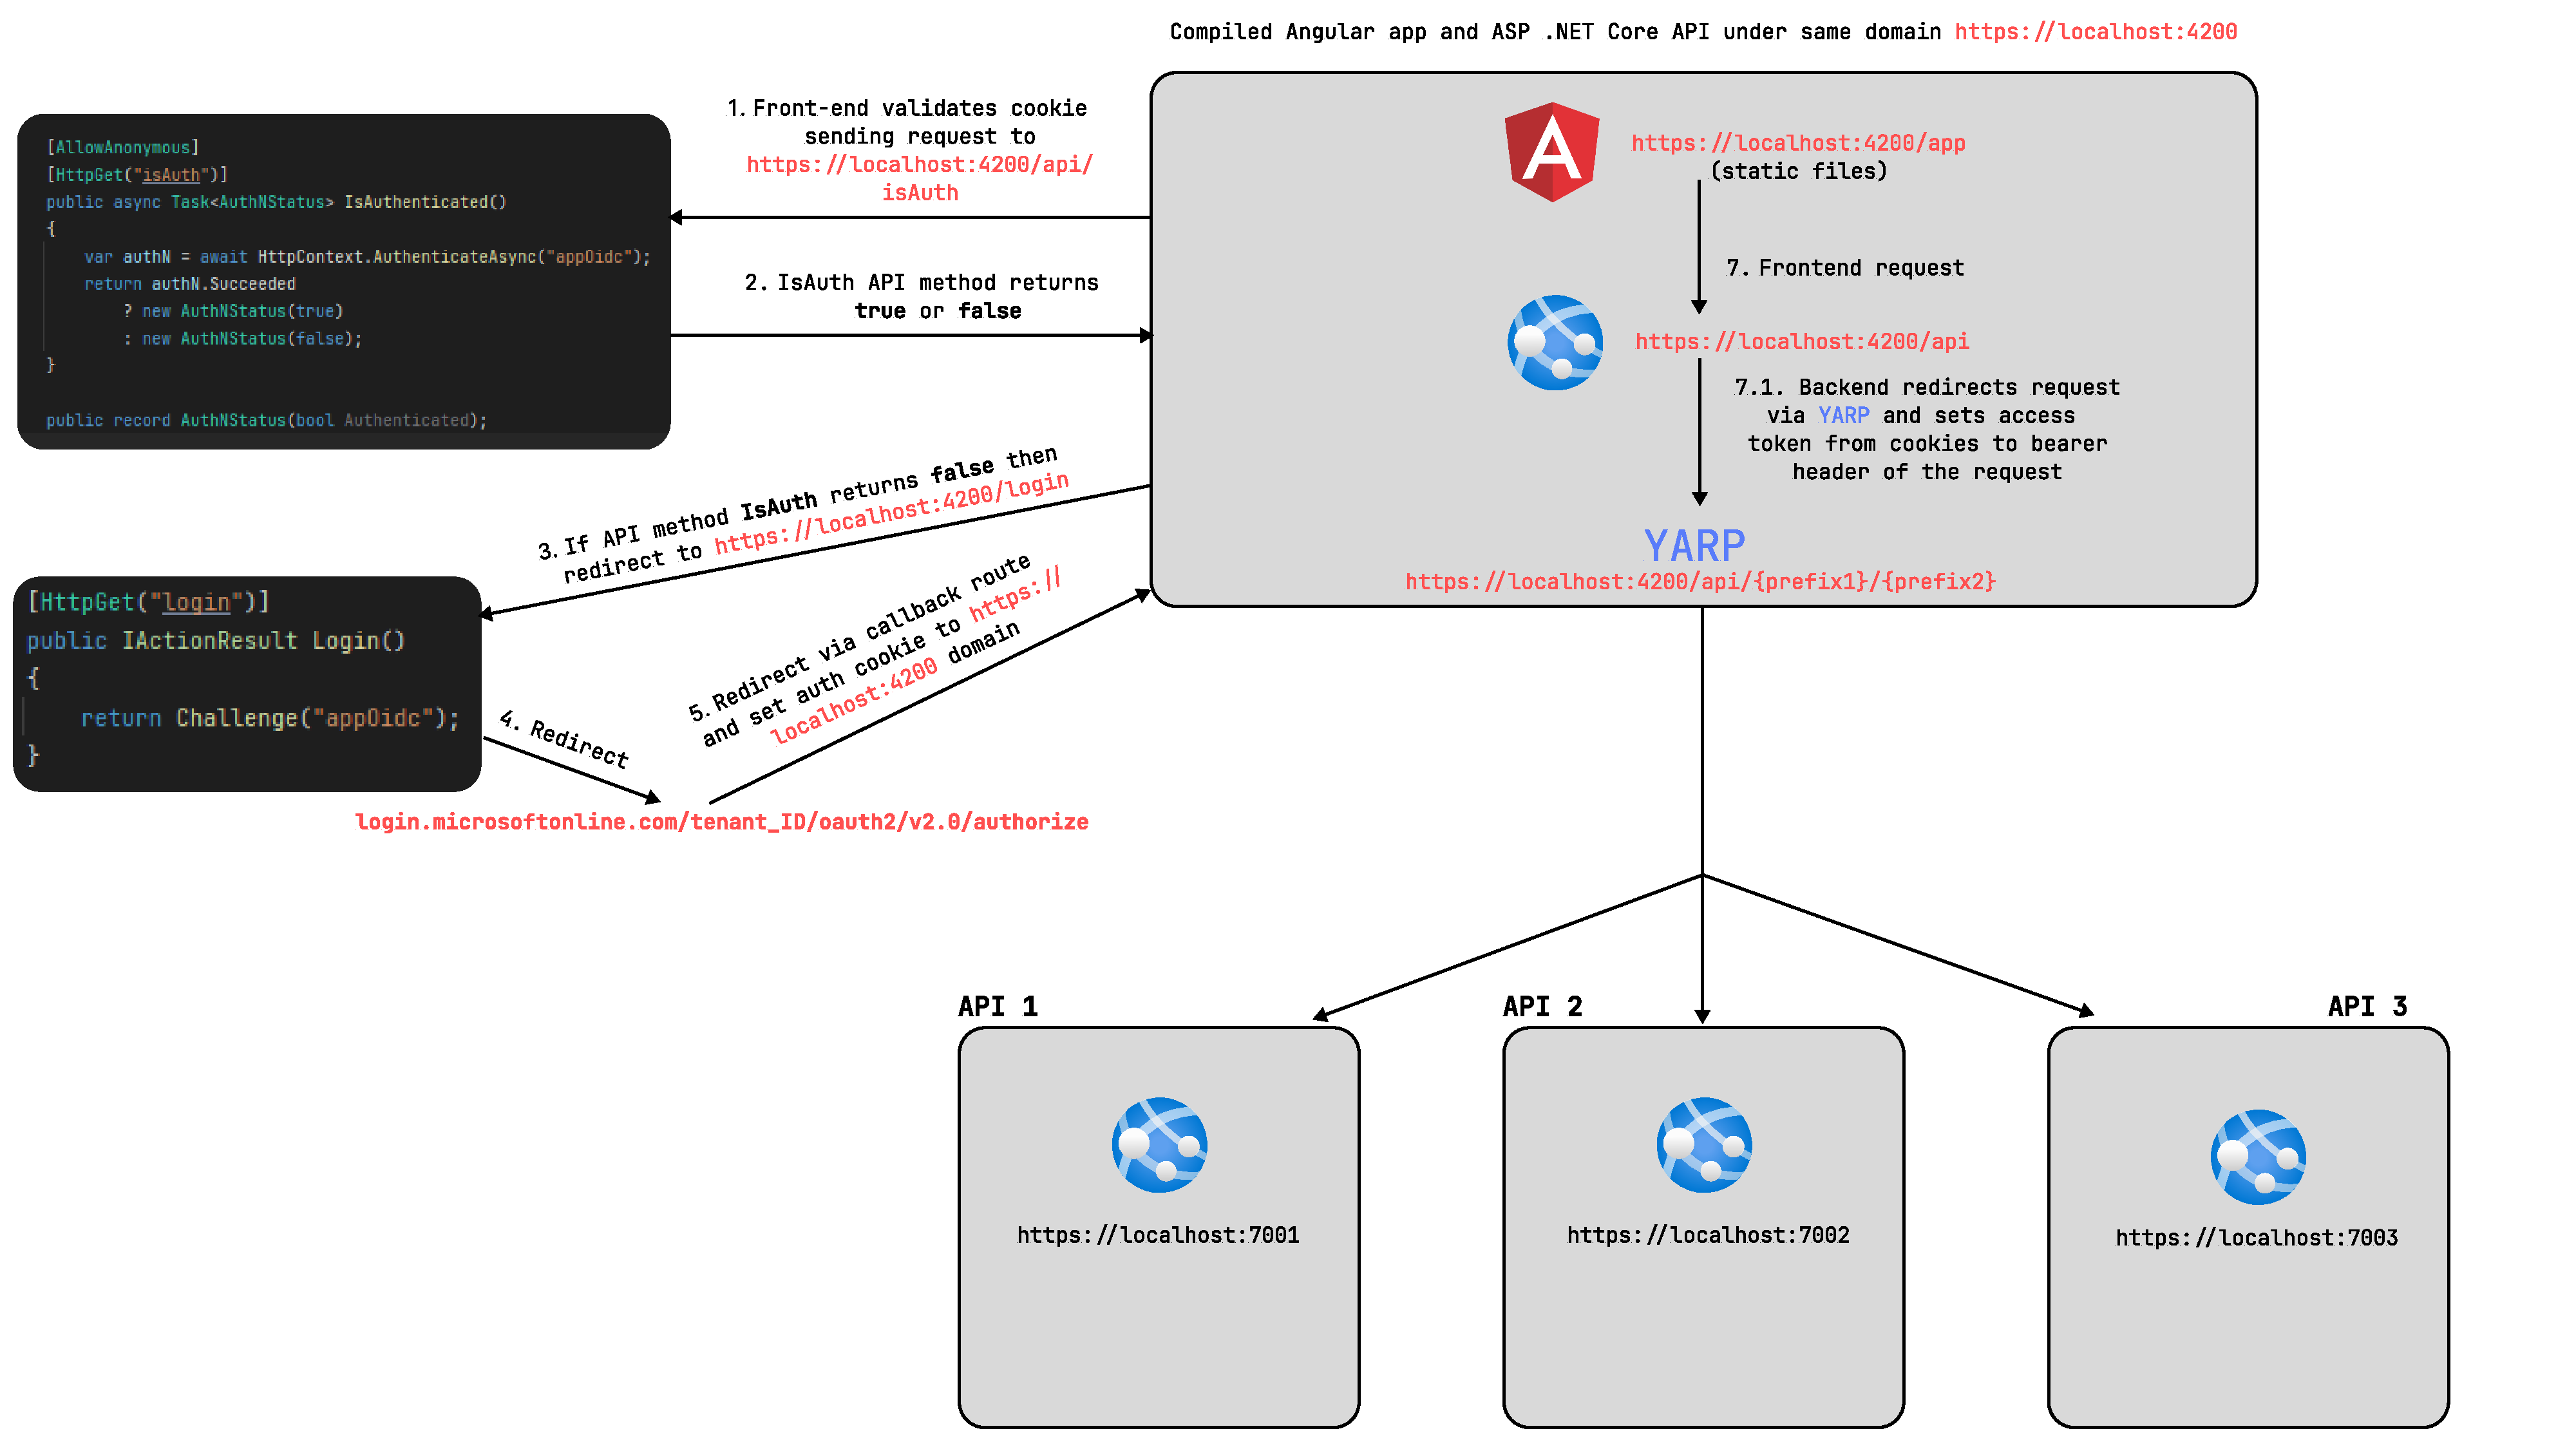
\includegraphics[width=1\textwidth]{img/Auth_flow_updated}
    ~\caption{Authentication flow diagram.}\label{fig:authentication_flow_diagram}
\end{figure}

Therefore, the whole authentication process can be described as eight steps such that
\begin{enumerate}
    \item Compiled Angular frontend application sends request to the authentication endpoint of the ASP .NET Core API
    to verify current authentication state.
    Angular application is a set of precompiled bundles that are exposed via same ASP .NET Core API at the \texttt{/app}
    endpoint so that cross-origin requests are not necessary and tokens can be stored in cookie files securely
    \item Authentication endpoint of the ASP .NET Core API responses either with
    HTTP status code \texttt{200 (OK)} or \texttt{401 (Unauthorized)}
    \item If \texttt{401 (Unauthorized)} status code received from previous step,
    then browser is redirected to the \texttt{login} endpoint of the ASP .NET Core API,
    otherwise user gets access to the protected resources
    \item Login method of the ASP .NET Core API redirects browser to the Azure AD authorize url
    \texttt{login.microsoftonline.com/tenant/oauth2/v2.0/authorize} where user enters his credentials.
    It is important to clarify that in order to get ID token we have to put parameter \texttt{openid} to the scope
    \begin{spverbatim}
    serviceCollection
    .AddAuthentication(options => {...})
    .AddCookie(CookieAuthenticationDefaults.AuthenticationScheme, options => {...})
    .AddOpenIdConnect(AuthConstants.AppOidc, options =>
        {
        ...
        options.Scope.Add("openid");
    });
\end{spverbatim}
    \item After successful authentication on the Azure AD side, the browser is redirected to the \texttt{fallback\_url}
    that is defined in Azure AD application registration.
    This \texttt{fallback\_url} is an active endpoint of the ASP .NET Core API\@.
    At this point, the \texttt{TickerStore}~\cite{microsoftIticketstore2023, ticketStore_2023}
    comes into the flow to manage user sessions.
    Each session is stored as a \texttt{UserSessionEntity} entity in the database.
    \begin{spverbatim}
    public class UserSessionEntity
    {
        public Guid Id { get; set; }
        public DateTimeOffset CreatedAt { get; set; }
        public DateTimeOffset ExpiresAt { get; set; }
        public DateTimeOffset UpdatedAt { get; set; }
        public DateTimeOffset DateOfLastAccess { get; set; }
        public byte[] Value { get; set; }
    }
\end{spverbatim}
    The Value property of type \texttt{byte[]} contains serialized \texttt{AuthenticationTicket}~\cite{microsoftAuthenticationTicket2023}
    object such that contains all required information like access, ID and refresh tokens.
    The class \texttt{TickerStore} implements \texttt{ITickerStore} interface that offers 4 methods:
    \texttt{StoreAsync, RenewAsync, RetrieveAsync, RemoveAsync}.
    \begin{itemize}
        \item The \texttt{StoreAsync} method is executed immediately after authentication on the authentication server,
        it saves the user session to the database.
        \item The \texttt{RenewAsync} method in our case is used by the background service to update user sessions.
        \item The \texttt{RetrieveAsync} method is executed every time a request is sent to the endpoint marked with the
        \texttt{[Authorize]} attribute.
        \item The \texttt{RemoveAsync} method is executed when the browser cookie has expired,
        as well as is used by the same \texttt{RefreshBackgroundService}
        to remove sessions which have not been used for a long time.
    \end{itemize}
    Example \texttt{TicketStore} implementation can be found at~\cite{ticketStore_2023}.
    Example of \texttt{TicketStore} dependency injection can be found at~\cite{ticketStoreDI_2023}.
    Authentication cookies are being setup at this step.
    \item Step 1 is repeated here, but now the HTTP request is for sure to be with \texttt{200 (OK)} status code.
    \item Precompiled Angular frontend application now sends request to the another microservice with authentication cookies
    attached to the request's \texttt{Bearer} header using \texttt{YARP} library~\cite{microsoftYarp2021},
    so that microservice is accessible.
    The \texttt{YARP} is configured according to~\cite{yarpDI_2023,yarpSectionAppSettings_2023}.
    \item If previous step returns \texttt{401 (Unauthorized)} status code, then Step 1 is repeated
\end{enumerate}